\section{Rappresentazione virtuale}

\subsection{Pybullet/URDF}

Inizialmente si era pensato di utilizzare la libreria Python Pybullet per creare l'ambiente tridimensionale, e un file .urdf.xacro per generare la mano.\\

Qui vengono riportate alcune immagini di tale prototipo virtuale.\\

\begin{figure}[htb] %width=0.6\linewidth
    \centering
    \subfloat
        {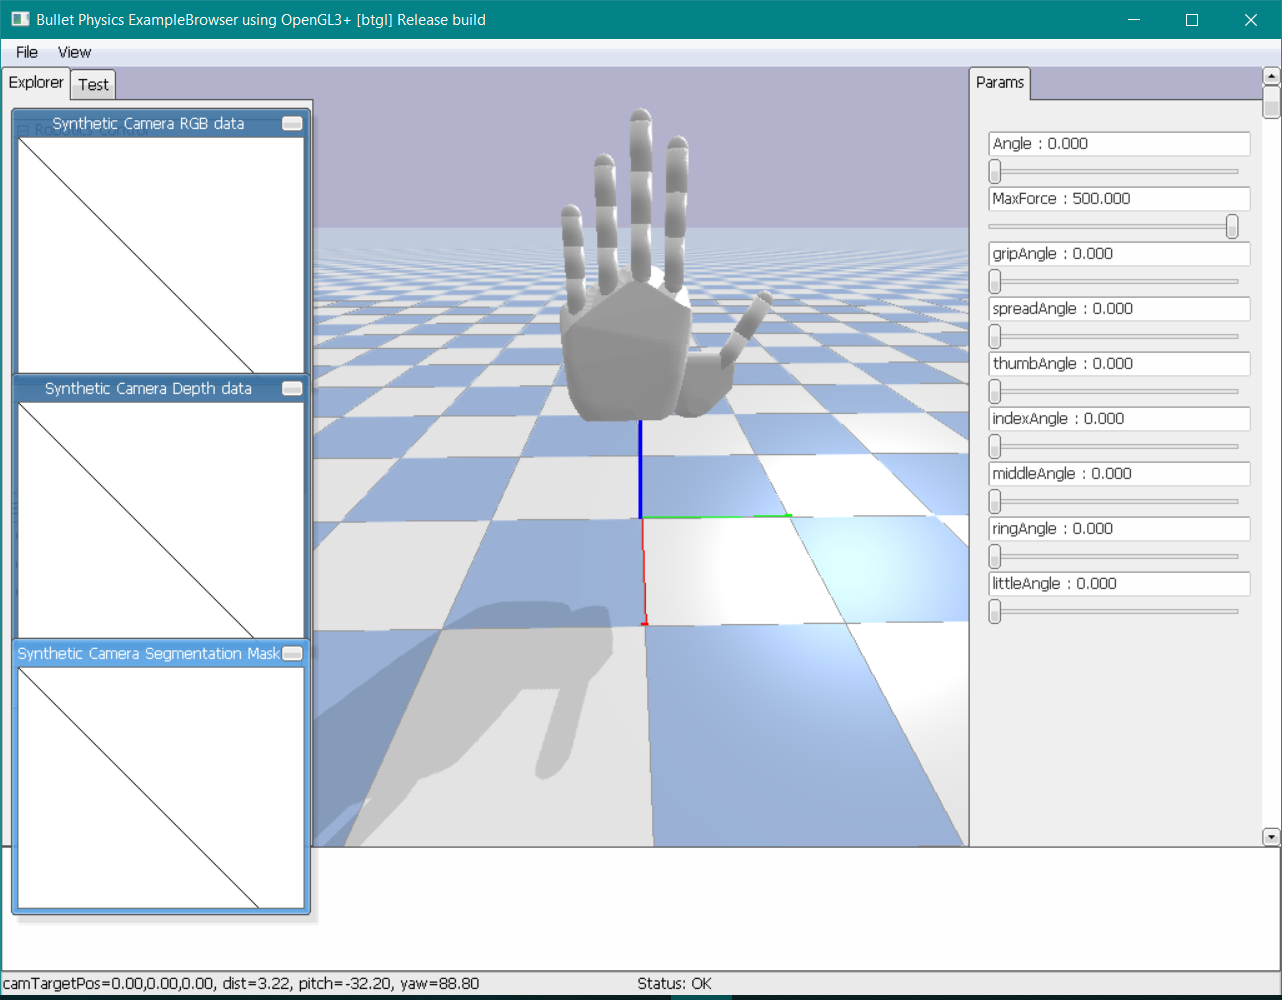
\includegraphics[height=.27\textheight]{immagini/pybullet urdf.PNG}}\
    \subfloat
        {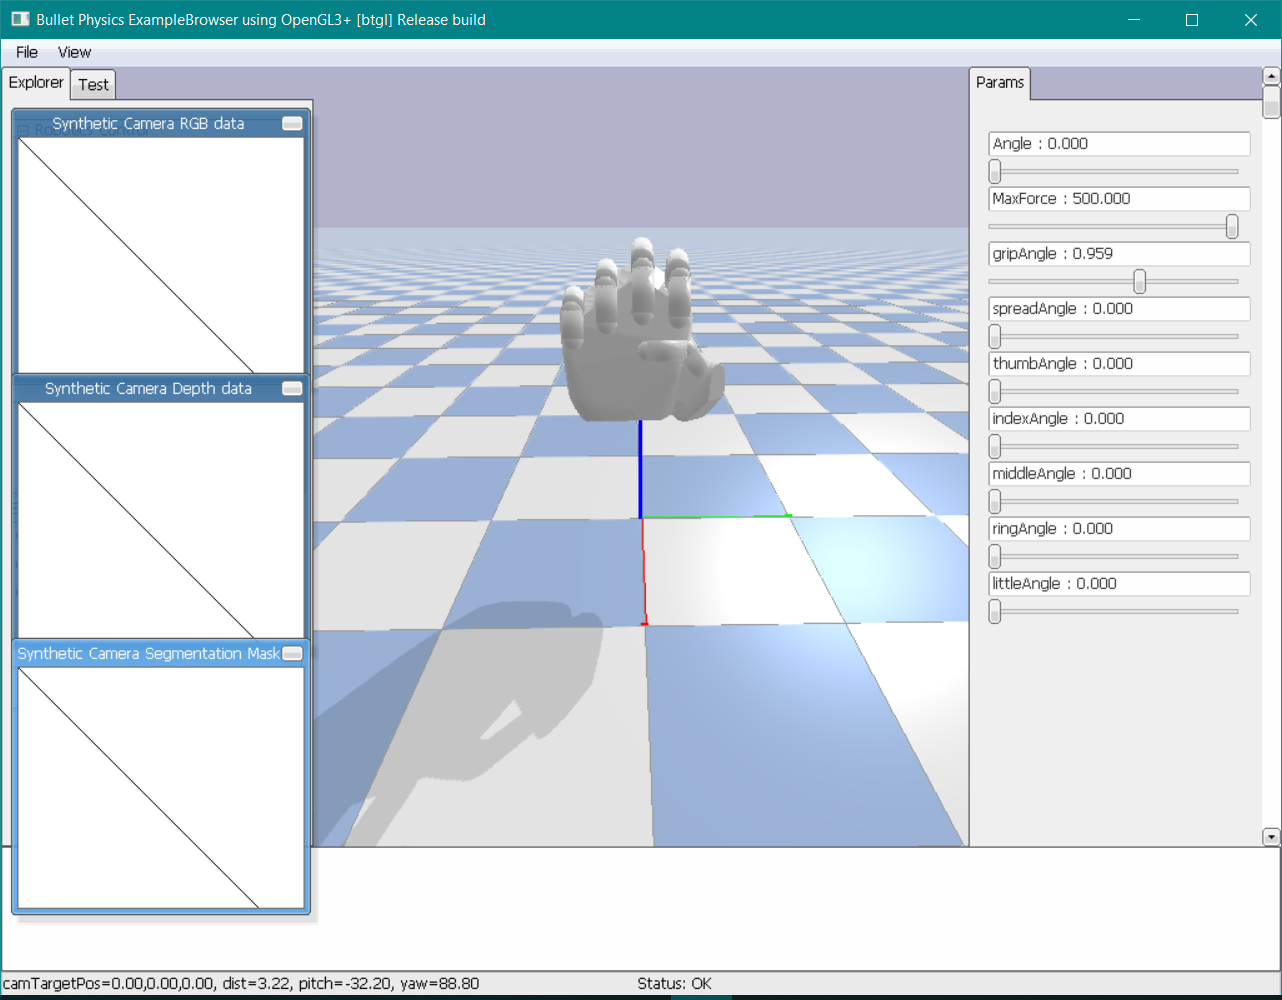
\includegraphics[height=.27\textheight]{immagini/pybullet urdf grip.PNG}}
    %\caption{}
\end{figure}

\begin{figure}[htb] %width=0.6\linewidth
    \centering
    \subfloat
        {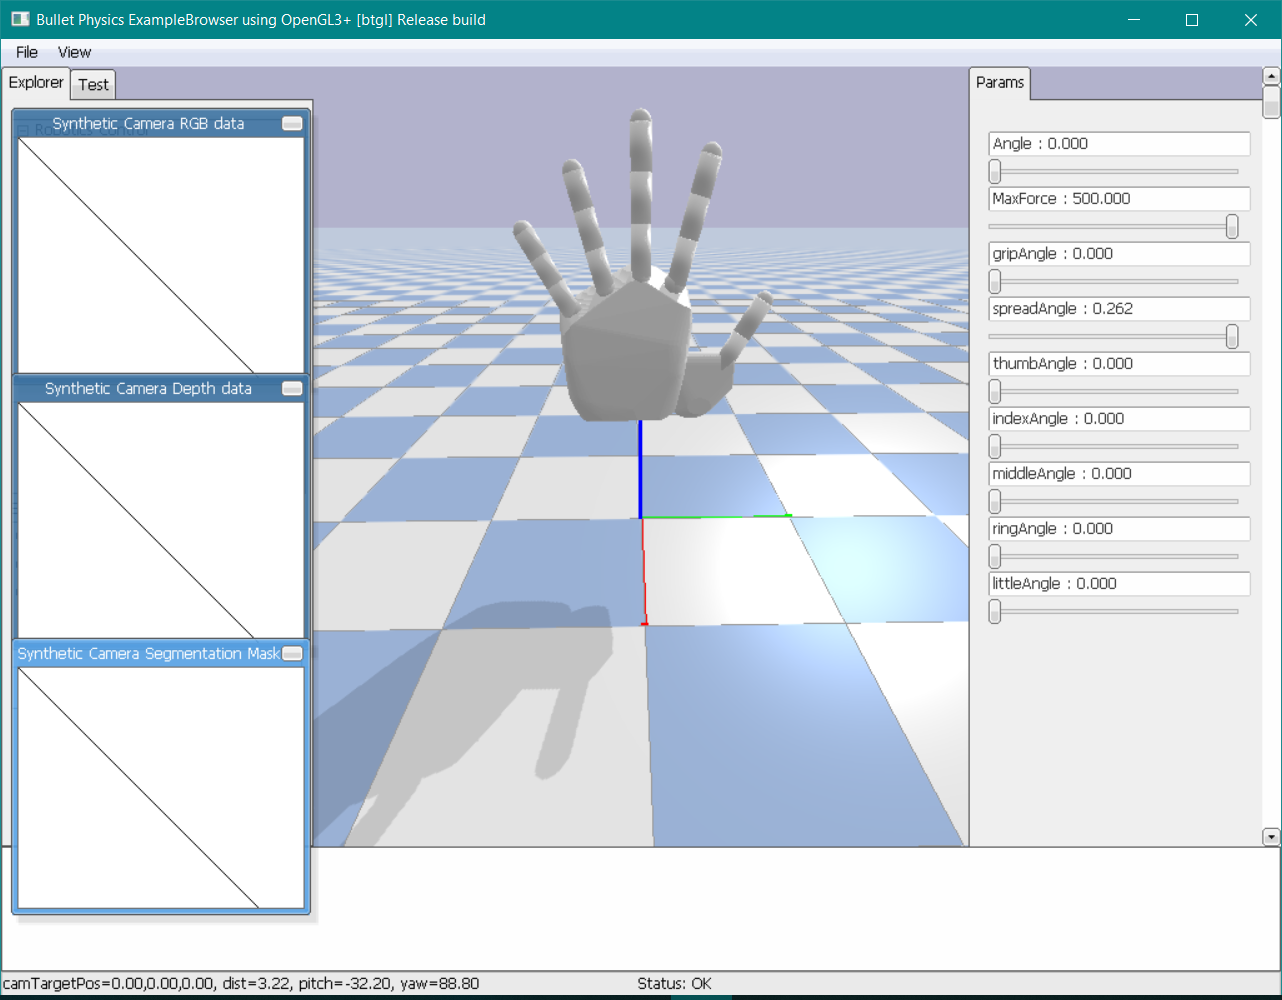
\includegraphics[height=.27\textheight]{immagini/pybullet urdf spread.PNG}}\
    \subfloat
        {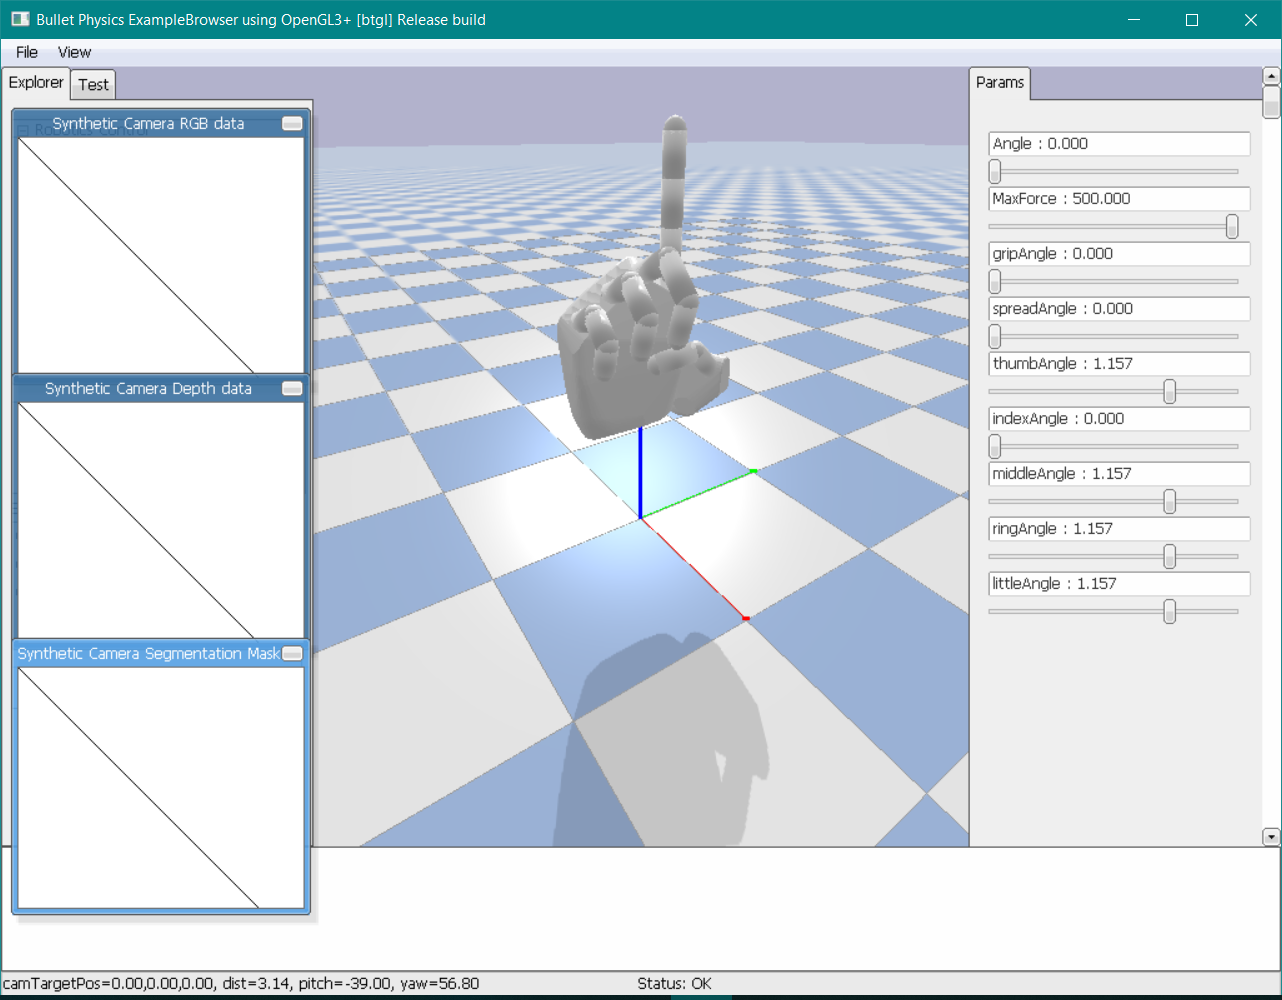
\includegraphics[height=.27\textheight]{immagini/pybullet urdf point.PNG}}
    %\caption{}
\end{figure}

\clearpage

\subsection{Unity}

In seguito si è passati all'utilizzo di Unity e alla mano virtuale dell'Oculus Rift.\\

\begin{figure}[H]
    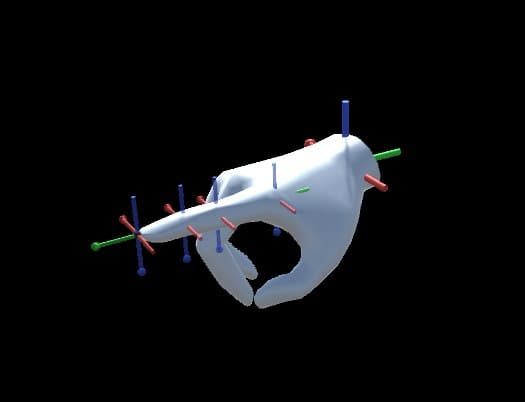
\includegraphics[scale=1]{immagini/vrhandunity.jpg}
    \centering
    \caption{Visualizzazione della mano su Unity}
\end{figure}

\\\\

\subsubsection{Elaborazione dei dati}

Una volta filtrati i dati tramite la batteria di stimatori d'assetto, vengono inviate le stime a una batteria di stimatori di orientazione relativa. Essi hanno lo scopo di calcolare l'angolo di giunto delle falangi della mano prendendo in ingresso l'assetto di 2 link successivi e calcolandone la rotazione relativa.

\begin{figure}[H]
    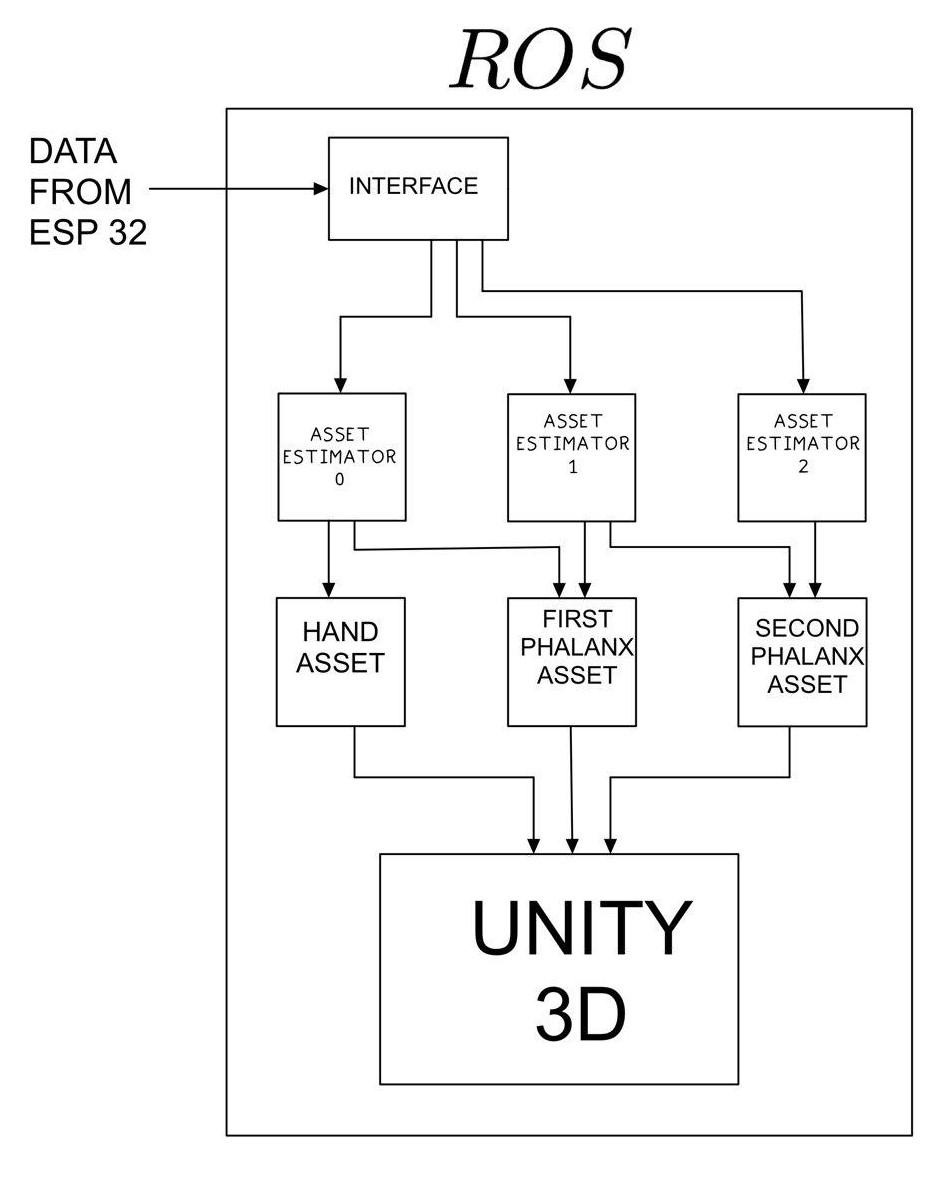
\includegraphics[scale=0.2]{immagini/unity.jpg}
    \centering
    \caption{Schema di stima e di calcolo di rotazioni relative}
\end{figure}

\begin{equation}
    T_{01_{rel}} = T_0(\theta_0,\phi_0,\psi_0)^{-1} \cdot T_1(\theta_1,\phi_1,\psi_1)
    \label{slerp}
\end{equation}

\begin{equation}
    T_{12_{rel}} = T_1(\theta_1,\phi_1,\psi_1)^{-1} \cdot T_2(\theta_2,\phi_2,\psi_2)
    \label{slerp}
\end{equation}\\

Dalla matrice di rotazione relativa possiamo estrapolare gli angoli di Eulero:
\begin{equation}
    R = T_{rel} =  \left(\begin{array}{ccc}
    r_{11}  & r_{12}  & r_{13} \\
    r_{21}  & r_{22}  & r_{23} \\
    r_{31}  & r_{32}  & r_{33} 
    \end{array}\right)
    \label{slerp}
\end{equation}\\\\
\begin{equation}
    phi = atan2(r_{23},r_{33})
\end{equation}\\\\
\begin{equation}
    theta = - arcsin(r_{13})
\end{equation}\\\\
\begin{equation}
    psi = atan2(r{12},r_{11})
\end{equation}\\

Una volta calcolati gli angoli di giunto vengono inviati tramite ROS2 i messaggi relativi ai singoli angoli di giunto e all'assetto della mano completa a un software di visualizzazione grafica. \\
Per validare i risultati è stata impostata una simulazione su Unity3D che ci permette di visualizzare in real time i risultati della stima d'asetto tramite codice C\# integrato in Unity. \\\\
Una volta che le stime degli angoli di giunto erano a disposizione su unity, i valori sono stati trasformati in quaternioni (i software di grafica 3D ne fanno uso estensivo visto il minor costo computazionale) e tra un campione e il successivo viene eseguita una interpolazione SLERP (spherical linear interpolation) di velocità programambile.\\
Essa è particolarmente indicata per interpolare grandezze di tipo angolare e migliora il risultato rendendo l'animazione più fluida e meno rumorosa.\\

\begin{equation}
    q = \begin{bmatrix}[1.5] \cos(\frac{\phi}{2})\cos(\frac{\theta}{2})\cos(\frac{\psi}{2}) + \sin(\frac{\phi}{2})\sin(\frac{\theta}{2})\sin(\frac{\psi}{2})\\ \sin(\frac{\phi}{2})\cos(\frac{\theta}{2})\cos(\frac{\psi}{2}) - \cos(\frac{\phi}{2})\sin(\frac{\theta}{2})\sin(\frac{\psi}{2})\\ \cos(\frac{\phi}{2})\sin(\frac{\theta}{2})\cos(\frac{\psi}{2}) + \sin(\frac{\phi}{2})\cos(\frac{\theta}{2})\sin(\frac{\psi}{2})\\ \cos(\frac{\phi}{2})\cos(\frac{\theta}{2})\sin(\frac{\psi}{2}) - \sin(\frac{\phi}{2})\sin(\frac{\theta}{2})\cos(\frac{\psi}{2}) \end{bmatrix}
\end{equation}

\begin{equation}
    Slerp(q_1,q_2,u) = q_1\cdot(q_1^{-1} \cdot q_2)^{u}
    \label{slerp}
\end{equation}

\begin{figure}[H]
    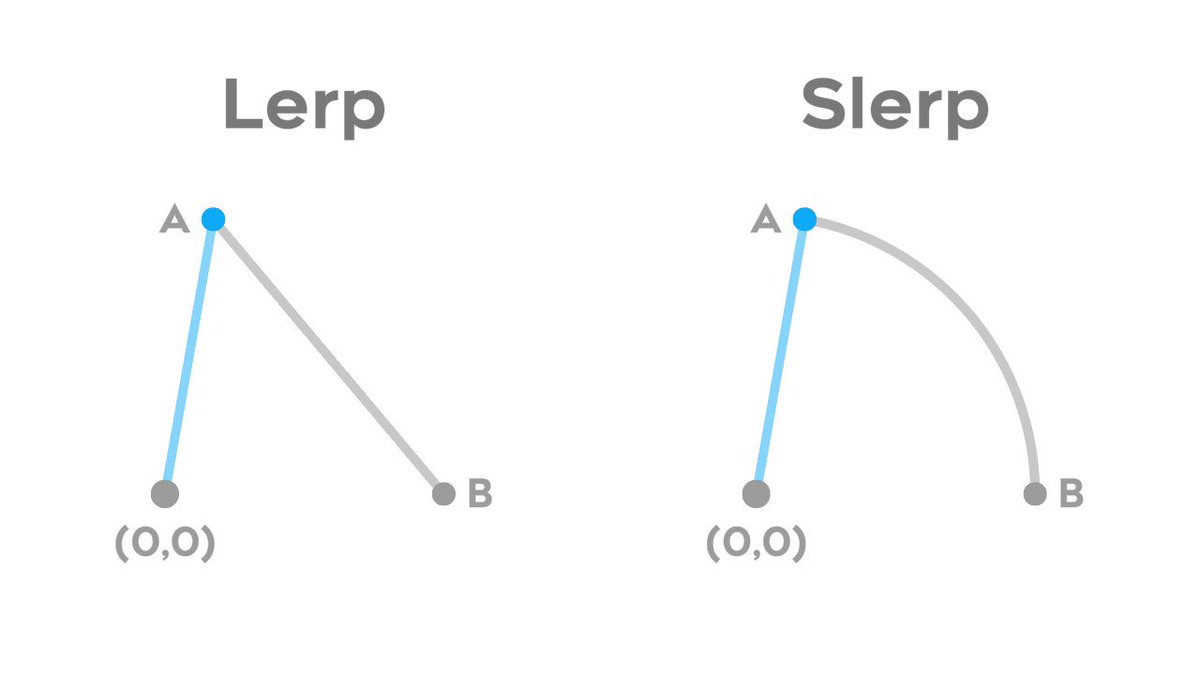
\includegraphics[scale=0.3]{immagini/lerp.jpg}
    \centering
    \caption{lerp - slerp piano}
\end{figure}

\begin{figure}[H]
    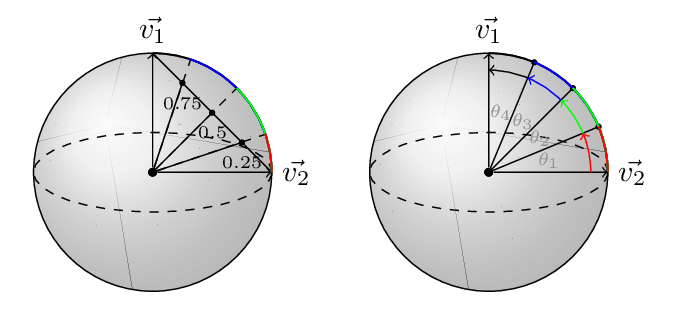
\includegraphics[scale=0.7]{immagini/slerplerp.png}
    \centering
    \caption{lerp - slerp differenza sulla sfera del quaternione unitario}
\end{figure}

È stata importata una mesh 3D di una mano da Oculus Rift, e ad essa sono stati agganciati sistemi di riferimento coerenti con quelli delle IMU.
I sistemi di riferimento vengono visualizzati secondo lo schema RGB - XYZ e sono solidali con i giunti presenti nella mano virtuale.

\begin{figure}[H]
    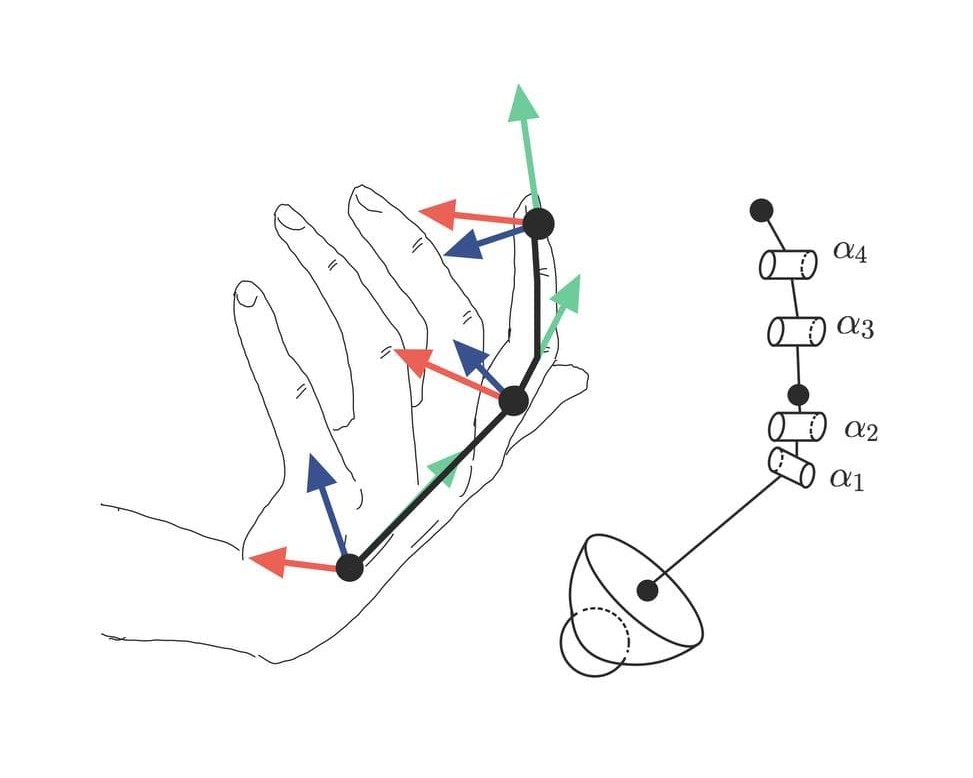
\includegraphics[scale=0.45]{immagini/kinematics_chain.jpg}
    \centering
    \caption{Catena cinematica.}
\end{figure}

Per la validazione dei risultati di stima abbiamo fatto uso esclusivamente di considerazioni di \textit{motion tracking}: muovendo il guanto, abbiamo considerato buona la stima quando la mano virtuale ne seguiva il movimento.

Per via delle convenzioni utilizzate al filtro e quelle usate da Unity la validità della simulazione risiede tra angoli compresi tra 0 e 180 gradi. Sforando questi angoli si hanno dei cambi di orientazione della mano.
Data la stima eccessivamente imprecisa dell'angolo $\alpha_1$ esso è stato mantenuto a 0.\\

\clearpage

\begin{figure}
 \centering
 \begin{subfigure}[ht]{0.3\textwidth}
     \centering
     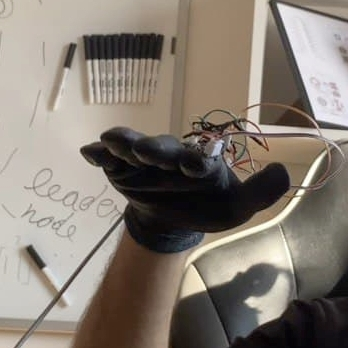
\includegraphics[width=5cm,height=5cm]{immagini/confronto/1.jpg}
     \caption{}
 \end{subfigure}
 \begin{subfigure}[ht]{0.3\textwidth}
     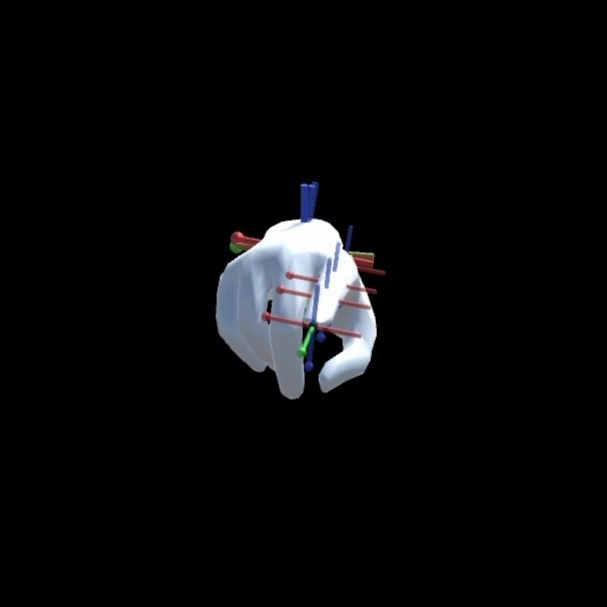
\includegraphics[width=5cm,height=5cm]{immagini/confronto/1_sym.jpg}
     \caption{}
 \end{subfigure}
 \caption{}
\end{figure}

\begin{figure}
 \centering
 \begin{subfigure}[ht]{0.3\textwidth}
     \centering
     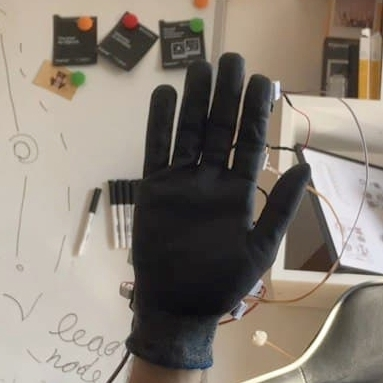
\includegraphics[width=5cm,height=5cm]{immagini/confronto/2_real.jpg}
     \caption{}
 \end{subfigure}
 \begin{subfigure}[ht]{0.3\textwidth}
     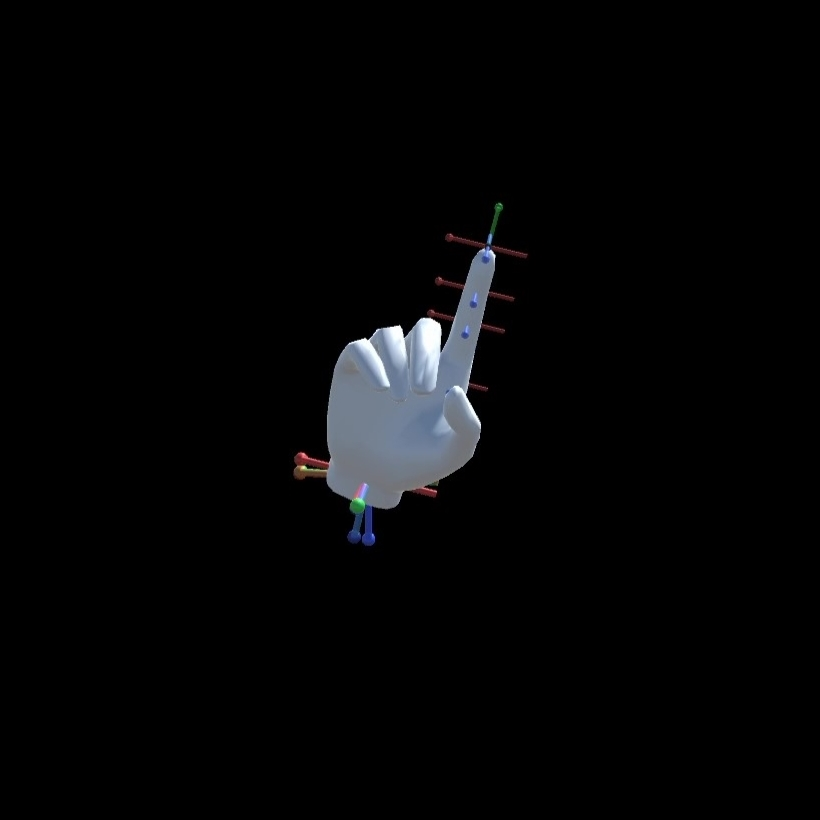
\includegraphics[width=5cm,height=5cm]{immagini/confronto/2_sym.jpg}
     \caption{}
 \end{subfigure}
 \caption{}
\end{figure}

\begin{figure}
 \centering
 \begin{subfigure}[ht]{0.3\textwidth}
     \centering
     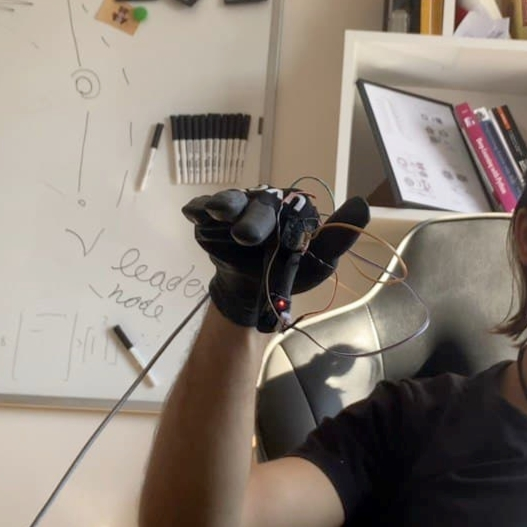
\includegraphics[width=5cm,height=5cm]{immagini/confronto/3_real.jpg}
     \caption{}
 \end{subfigure}
 \begin{subfigure}[ht]{0.3\textwidth}
     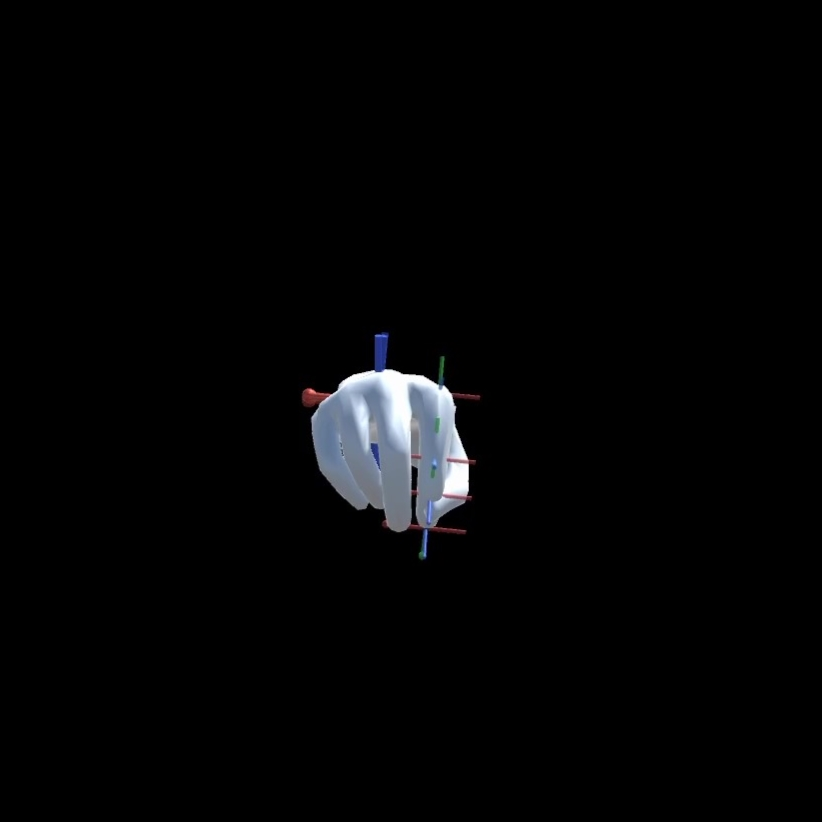
\includegraphics[width=5cm,height=5cm]{immagini/confronto/3_sym.jpg}
     \caption{}
 \end{subfigure}
 \caption{}
\end{figure}

\begin{figure}
 \centering
 \begin{subfigure}[ht]{0.3\textwidth}
     \centering
     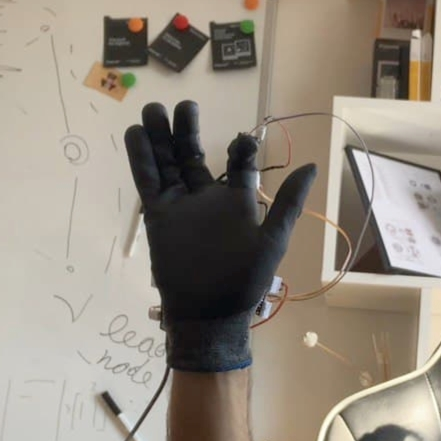
\includegraphics[width=5cm,height=5cm]{immagini/confronto/4_real.jpg}
     \caption{}
 \end{subfigure}
 \begin{subfigure}[ht]{0.3\textwidth}
     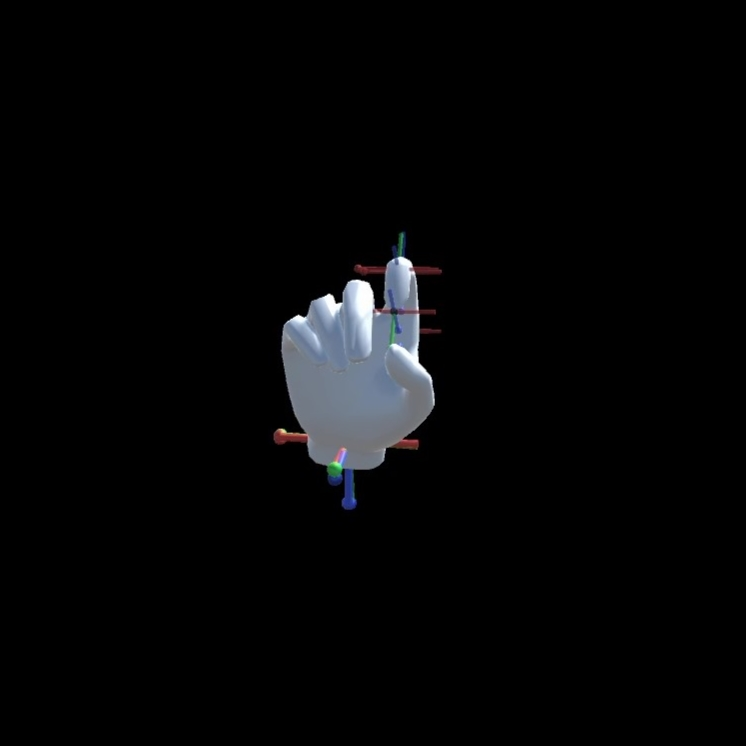
\includegraphics[width=5cm,height=5cm]{immagini/confronto/4_sym.jpg}
     \caption{}
 \end{subfigure}
 \caption{}
\end{figure}

\begin{figure}
 \centering
 \begin{subfigure}[ht]{0.3\textwidth}
     \centering
     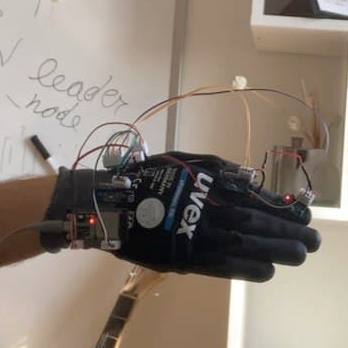
\includegraphics[width=5cm,height=5cm]{immagini/confronto/5_real.jpg}
     \caption{}
 \end{subfigure}
 \begin{subfigure}[ht]{0.3\textwidth}
     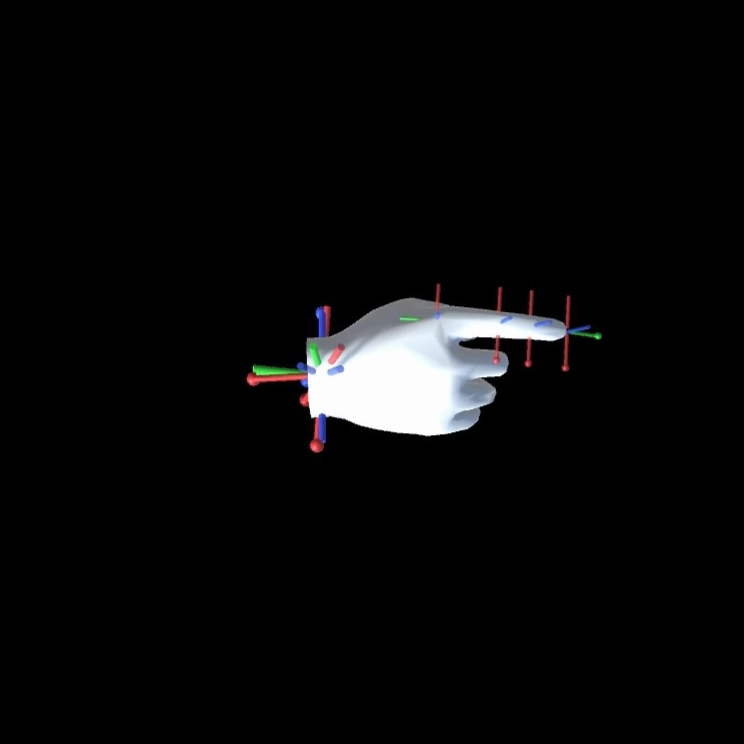
\includegraphics[width=5cm,height=5cm]{immagini/confronto/5_sym.jpg}
     \caption{}
 \end{subfigure}
 \caption{}
\end{figure}

\begin{figure}
 \centering
 \begin{subfigure}[ht]{0.3\textwidth}
     \centering
     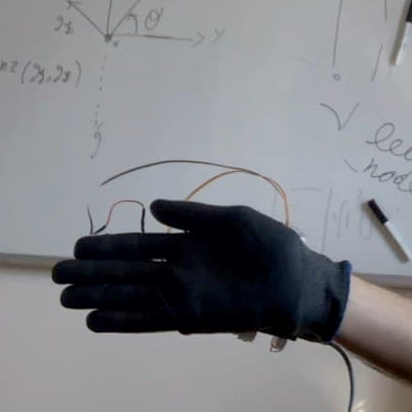
\includegraphics[width=5cm,height=5cm]{immagini/confronto/6_real.jpg}
     \caption{}
 \end{subfigure}
 \begin{subfigure}[ht]{0.3\textwidth}
     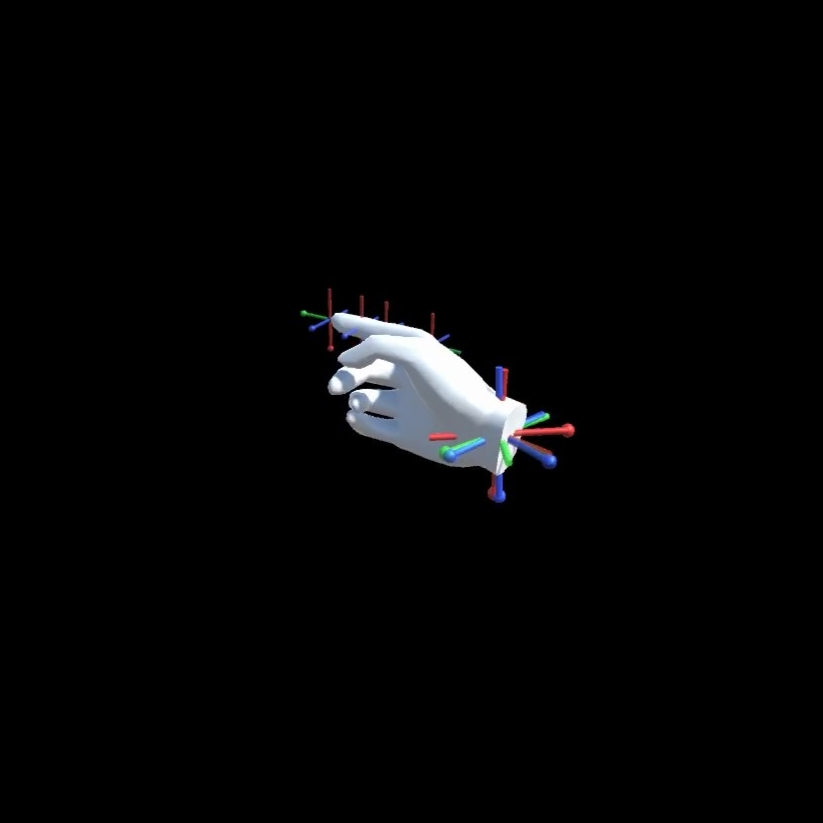
\includegraphics[width=5cm,height=5cm]{immagini/confronto/6_sym.jpg}
     \caption{}
 \end{subfigure}
 \caption{}
\end{figure}

\begin{figure}
 \centering
 \begin{subfigure}[ht]{0.3\textwidth}
     \centering
     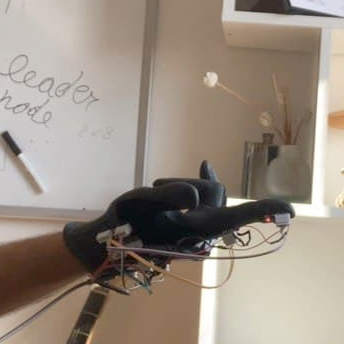
\includegraphics[width=5cm,height=5cm]{immagini/confronto/7_real.jpg}
     \caption{}
 \end{subfigure}
 \begin{subfigure}[ht]{0.3\textwidth}
     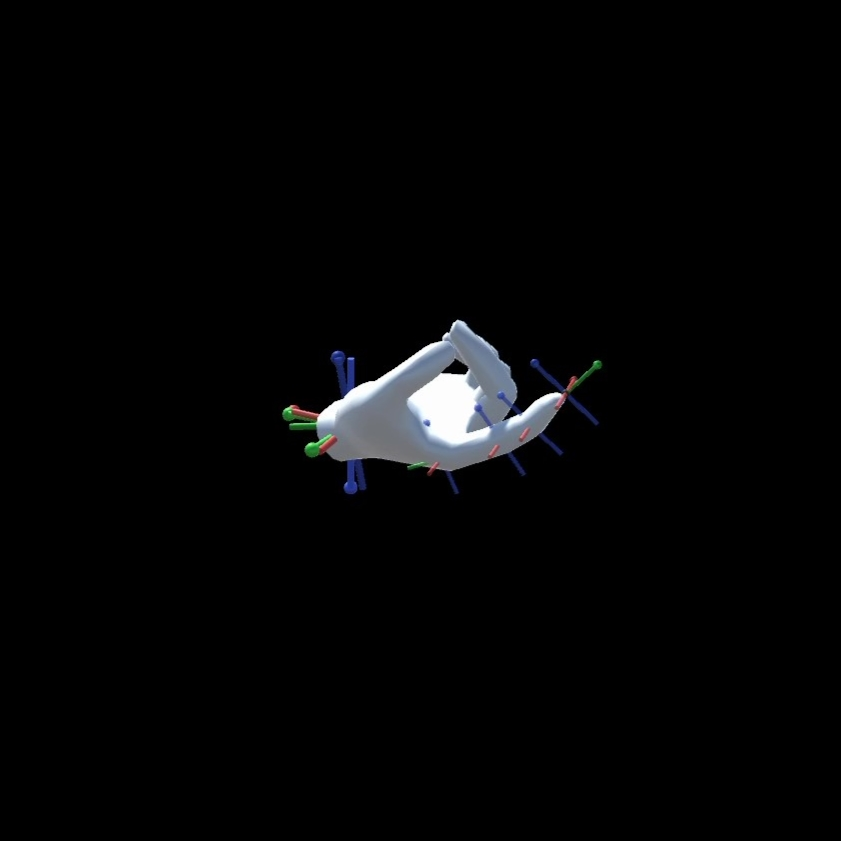
\includegraphics[width=5cm,height=5cm]{immagini/confronto/7_sym.jpg}
     \caption{}
 \end{subfigure}
 \caption{}
\end{figure}

\begin{figure}
 \centering
 \begin{subfigure}[ht]{0.3\textwidth}
     \centering
     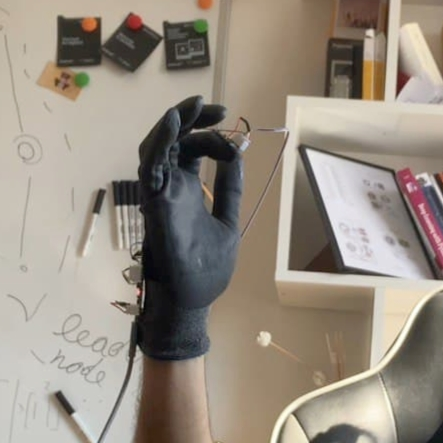
\includegraphics[width=5cm,height=5cm]{immagini/confronto/8_real.jpg}
     \caption{}
 \end{subfigure}
 \begin{subfigure}[ht]{0.3\textwidth}
     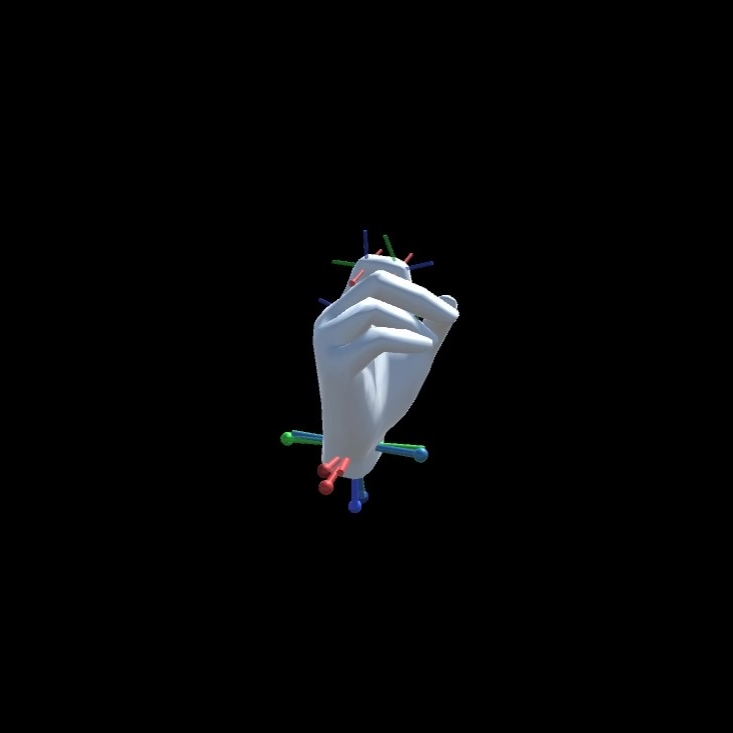
\includegraphics[width=5cm,height=5cm]{immagini/confronto/8_sym.jpg}
     \caption{}
 \end{subfigure}
 \caption{}
\end{figure}


\clearpage